\subsection{Problem}

\renewcommand{\theequation}{\theenumi}
\begin{enumerate}[label=\thesection.\arabic*.,ref=\thesection.\theenumi]
\numberwithin{equation}{enumi}
	\item Find the angle between the x-axis and the line joining the points 
	\begin{align}
\vec{A} = \myvec{3\\-1}\text{ and }\vec{B} = \myvec{4\\-2}.
	\end{align}
	The following python code computes the angle which the line in Fig.\ref{fig:qnine} makes with x-axis.
	\begin{lstlisting}
	./codes/lines/q9.py
	\end{lstlisting}
	
	\solution The slope of line $\vec{AB}$ is given as:
	\begin{align}
\tan \theta = \frac{B[1]-A[1]}{B[0]-A[0]}
		\\
\text{which on computing yields} \quad \tan \theta = -1
\\
\therefore \theta = \tan^{-1}(-1) = 135\degree	
	\end{align}

	\begin{figure}[!ht]
	\centering
	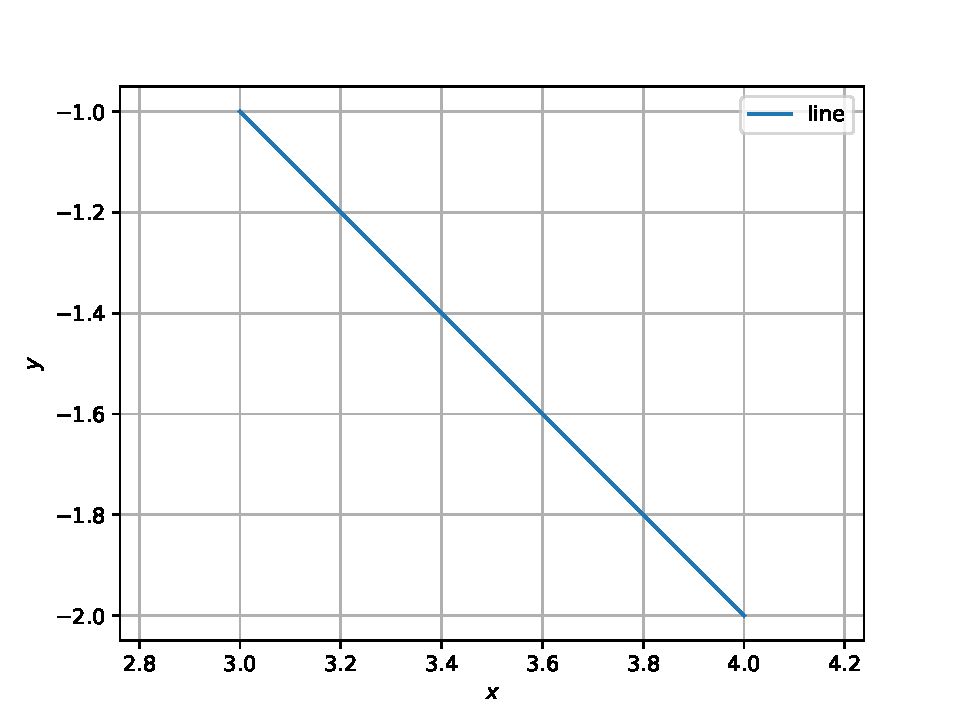
\includegraphics[width=\columnwidth]{./figs/lines/q9.pdf}
	\caption{Line of Q.3.5.5}
	\label{fig:qnine}	
	\end{figure}
	
\end{enumerate}

